\documentclass{beamer}
\usepackage[citestyle=ieee, style=ieee, backend=biber, giveninits=true]{biblatex}
\usepackage{lmodern}
\usepackage{amsmath}
\usepackage{mathtools}
\usepackage[version=3]{mhchem} % Formula subscripts using \ce{}, e.g., \ce{H2SO4}
\usepackage{siunitx}
\usepackage{hyperref}
\usepackage[utf8]{inputenc}

\graphicspath{{./Figures/}}

% clear title and doi from citations
% from https://tex.stackexchange.com/q/165481/56227
\AtEveryCitekey{\clearfield{doi}\clearfield{title}}

% use dash for range phrase by default, and one unit
\sisetup{range-phrase=--, range-units = single}

%smaller footnotes, adapted from http://tex.stackexchange.com/a/146021
\setbeamerfont{footnote}{size=\fontsize{7pt}{0pt}}

%footnote spacing avoids navigation / margins, adapted from http://tex.stackexchange.com/a/44231
\addtobeamertemplate{footnote}{\vspace{-6pt}\advance\hsize-0.5cm}{\vspace{6pt}}
\makeatletter
% Alternative A: footnote rule
\renewcommand*{\footnoterule}{\kern -3pt \hrule \@width 2in \kern 8.6pt}
% Alternative B: no footnote rule
% \renewcommand*{\footnoterule}{\kern 6pt}
\makeatother

%make frame for each section
\AtBeginSection[]{
  \begin{frame}
  \vfill
  \centering
  \begin{beamercolorbox}[sep=8pt,center,shadow=true,rounded=true]{title}
    \usebeamerfont{title}\insertsectionhead\par%
  \end{beamercolorbox}
  \vfill
  \end{frame}
}

\newcounter{dummynote1}% Save footnote counter
\newcounter{dummynote2}% Save footnote counter

%auto incrementing titles from http://tex.stackexchange.com/a/231533
\newcounter{expensive}
\newcommand\ExpTitle{%
  \frametitle{\refstepcounter{expensive}{Chemical kinetic integration is \textbf{expensive}}~\theexpensive}}
\resetcounteronoverlays{expensive}

\newcounter{rosen}
\newcommand\RosenTitle{%
  \frametitle{\refstepcounter{rosen}{Rosenbrock Methods}~\therosen}}
\resetcounteronoverlays{rosen}

\newcounter{wmeth}
\newcommand\WTitle{%
  \frametitle{\refstepcounter{wmeth}{W-Methods}~\thewmeth}}
\resetcounteronoverlays{wmeth}

\newcounter{twostep}
\newcommand\TwoStepTitle{%
  \frametitle{\refstepcounter{twostep}{Two-Step Rosenbrock-type Methods}~\thetwostep}}
\resetcounteronoverlays{twostep}

\newcounter{stiff}
\newcommand\BalanceTitle{%
  \frametitle{\refstepcounter{stiff}{Stiffness-based Load Balancing}~\thestiff}}
\resetcounteronoverlays{stiff}

\bibliography{lit_review.bib}

%opening
\title{Accelerating chemical kinetic integration for reacting-flows on hybrid architectures: A Literature Review}
\author{Nick Curtis}
\institute{University of Connecticut}
\date{\today}

\begin{document}

\maketitle

\section{Introduction}

\begin{frame}
\frametitle{Realistic chemical modeling is \textbf{critical}}
In order to meet increasingly stringent emissions and efficiency requirements, designers of combustion devices have turned to \textbf{new technologies} and \textbf{new fuels}
\begin{itemize}
 \item Novel combustion regimes such as low-temperature combustion are often controlled by chemical processes, rather than directly controllable physical processes as in current technology
 \item Further, developed solutions must be flexible to accommodate a variety of next generation fuels
\end{itemize}
Computationally guided combustion design has played an important role in development of these new technologies, however use of realistic chemical modeling (as required for predictive reacting-flow simulations) is prohibitively expensive for most practical systems. 
\end{frame}

\begin{frame}
 \frametitle{Chemical kinetic integration is \textbf{expensive}}
 The size of chemical kinetic models for fuels relevant transportation and energy generation may consist of hundreds to thousands of chemical species, with potentially tens of thousands of reactions.
 \begin{itemize}
  \item e.g., for gasoline \footfullcite{Mehl:2011cn} and jet fuel\footfullcite{Naik2011434}
 \end{itemize}
 Further, chemical kinetic models are typically \textbf{stiff}---due to the presence of highly reactive radicals and associated short chemical timescales.
 \begin{itemize}
  \item Typically implicit integration techniques are used to efficiently deal with stiffness, requiring repeated evaluation and factorization of the chemical kinetic Jacobian.
  \item Naive implementations of these operations scale \textbf{quadratically} and \textbf{cubically} with the number of species in a model, respectively\footfullcite{Lu:2009gh}.
 \end{itemize}
\end{frame}

%\begin{frame}
% \ExpTitle
% As a result, chemical kinetic integration may be the most computationally intensive portion of reacting flow simulations, e.g. consuming \SI{70}{\percent}~\footfullcite{kodavasal2016development} of the total solver time in each time-step.
%\end{frame}


\begin{frame}
 \frametitle{Strategies for cost reduction}
 A few of the major strategies to accelerate chemical kinetic integration:
 \begin{itemize}
  \item \textbf{Model reduction}, a host of techniques to reduce the size of the system being solved while maintaining accurate chemical kinetics (as compared to the full model)
  \item \textbf{Improved integration techniques}, development of new integration algorithms specifically for chemical kinetics, e.g. hybrid implicit\slash explicit integrators, tabulation techniques, analytical Jacobian codes, and on-the-fly stiffness removal
  \item \textbf{Solver vectorization}, to better utilize available hardware, e.g. via single-instruction, multiple-data (or multiple-thread) (SIMD\slash SIMT) execution on central processing units (CPUs) and other accelerators such as Intel's many integrated core architecture (MIC) or graphics processing units (GPUs).
  \item \textbf{High performance computing techniques}, stiffness-based load balancing, scaling for high performance clusters
 \end{itemize}
 We will focus on (SIMD) \textbf{vectorization}, \textbf{improved integration} and \textbf{high performance computing} techniques.
\end{frame}

\begin{frame}
 \frametitle{Operator splitting and vectorization}
 Most reacting-flow codes utilize the operator-splitting techniques (e.g.~\footfullcite{Knio:1999}$^{,}$~\footfullcite{Ren:2008}), separating a large system of coupled partial differential equations (PDEs), such that different physical processes are solved independently.
 \begin{itemize}
  \item Stiff integration technique used for chemical kinetics, and an explicit scheme for transport, etc.
  \item Avoids the high cost of solving the fully coupled PDEs
  \item Independent initial value problem (IVP) of chemical kinetic ordinary differential equations (ODEs) at each computational location (e.g. cell) in the domain~$\rightarrow$~vectorization!
 \end{itemize}
 It is noted that significant error can be introduced by operator-splitting schemes if the time-steps are not chosen properly~\footfullcite{Gao2015287}.
\end{frame}

\section{Single Instruction, Multiple Data\slash Thread Processing Paradigms}

\begin{frame}
 \frametitle{Single instruction, multiple data processing}
 \setcounter{dummynote1}{\value{footnote}}
 \addtocounter{dummynote1}{1}
 \begin{columns}
 \begin{column}{0.6\textwidth}
  \textbf{SIMD} computing is a vectorization paradigm that allows processing elements (PE)---e.g a CPU core---to execute the same instruction concurrently on different data.
  \begin{itemize}
    \item Each vector unit contains multiple processing units (PUs), which together are called a \textbf{vector lane}
    \item Each vector unit operates on a \textbf{superword}, a variable length data array---usually, \numrange{2}{16} double precision floats (doubles)
    \item Typically a single thread resides on each PE and issues SIMD vector instructions over multiple data
    %\begin{itemize}
    % \item It is possible to have multiple threads per PE, but SIMD instructions between threads do not interact
    %\end{itemize}
  \end{itemize}
 \end{column}
 \begin{column}{0.4\textwidth}
  \begin{figure}
    \centering
    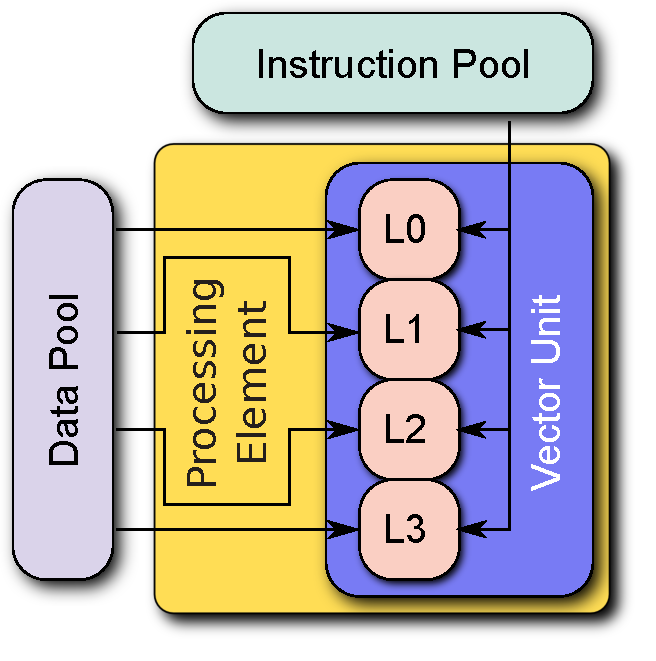
\includegraphics[width=\columnwidth]{SIMD.pdf}
    \caption{Schematic of SIMD processing.  Adapted from\footnotemark[\value{dummynote1}]}
  \end{figure}
 \end{column}
 \footnotetext[\value{dummynote1}]{\fullcite{Simdfig:2016}}
 \end{columns}
 \setcounter{footnote}{\value{dummynote1}}
\end{frame}

\begin{frame}
 \frametitle{Single instruction, multiple thread processing}
 \begin{columns}
 \begin{column}{0.6\textwidth}
 \textbf{SIMT} processing is a related, though separate concept.
 \begin{itemize}
  \item Multiple threads reside on a PE, each with instructions to execute at each step (e.g., \textrm{I1}, \textrm{I2} in figure)
  \item All threads that need to execute the same instruction (e.g. \textrm{I1}) execute simultaneously
  \item If some threads need a different instruction (e.g. \textrm{I2}), they must wait and execute their instruction after the other threads
  \item This is known as \textbf{thread divergence}, and is an important performance concern.
 \end{itemize}
 \end{column}
 \begin{column}{0.4\textwidth}
  \begin{figure}[r]
    \centering
    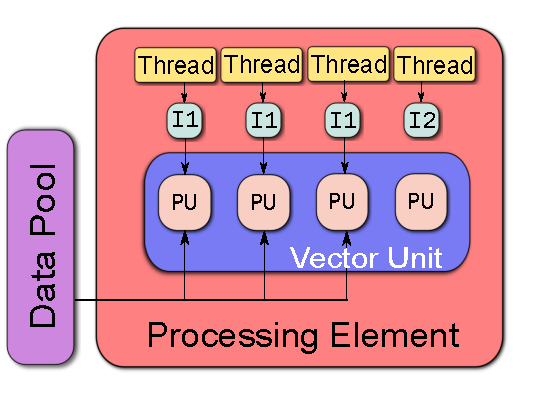
\includegraphics[width=\columnwidth]{SIMT.pdf}
    \caption{Schematic of SIMT processing}
  \end{figure}
 \end{column}
 \end{columns}
\end{frame}

    
\begin{frame}
 \frametitle{CPU-based SIMD computing for chemical kinetic integration}
 Most modern GPUs are based on a SIMT architecture~\footfullcite{lindholm2008nvidia}, while all modern CPUs and some accelerators (e.g., the MIC) contain SIMD processors.
 For SIMD computing, different levels of parallelism are available:
 \begin{itemize}
  \item Multiple PEs (e.g., multiple cores)
  \item SIMD processing available within each PE
  \item Additionally, multiple threads may reside on PE (e.g., a \textit{hyperthreaded} CPU core)
 \end{itemize}
 Different levels of SIMD cooperation possible:
 \begin{itemize}
  \item Each chemical kinetic IVP is assigned to separate SIMD lane, meaning a PE solves multiple IVPs $\rightarrow$ \textbf{shallow} vectorization
  \item Each PE uses SIMD operators to vectorize solution of a single IVP $\rightarrow$ \textbf{deep} vectorization
 \end{itemize}
\end{frame}

\begin{frame}
  \frametitle{CPU-based SIMD Computing -- Difficulties}
  Explicit use of SIMD instructions is typically platform--dependent and difficult to implement~\footfullcite{Stone:2016}.
  \begin{itemize}
   \item Specialized compilers are often used to identify vectorizable loops and generate the appropriate platform--dependent SIMD code.
  \end{itemize}
  Recently many tools have emerged to ease the development burden of SIMD programming
  \begin{itemize}
   \item \texttt{OpenCL}~\footfullcite{Stone:2010} is a platform--independent language geared towards SIMT\slash SIMD programming.
   \item \texttt{loo.py}~\footfullcite{Klockner:2014} is a python--based code generation platform that generates SIMT\slash SIMD code for CPUs and GPUs and other accelerators, e.g., Intel's Many Integrated Core (MIC) processor
  \end{itemize}
\end{frame}

\section{CPU-based SIMD Integration of Stiff IVPs}

\begin{frame}[allowframebreaks]
 \frametitle{Comparison of SIMD and SIMT parallelization on multiple platforms}
 Stone and Niemeyer~\footfullcite{Stone:2016} investigated the speedup of shallow SIMD\slash SIMT vectorizations of two fourth-order integration techniques on the CPU\footnote{using AVX (128-bit) vector instructions}, GPU and an Intel Xeon Phi co-processor (MIC) over a baseline multithreaded OpenMP code that was deep-vectorized via compiler pragmas.
 \begin{itemize}
  \item A non-stiff explicit Rungke-Kutta-Fehlberg and stiff linearly-implicit\footnote{A linearly implicit integrator does not require Newton-Iteration} Rosenbrock scheme were used
  \item Speedups of \SIrange{2.2}{3}{\times} were achieved for chemical kinetic rate evaluation using shallow-vectorized CPU, GPU and MIC codes
  \item Speedups of up to \SI{1.4}{\times}, \SI{2.5}{\times} and \SI{3.2}{\times} were found for the Rosenbrock solver on the GPU, CPU, and MIC respectively.
  \item Thread divergence may cause significant performance degradation for the GPU solvers
 \end{itemize}
\end{frame}

\begin{frame}
 \frametitle{Shallow-SIMD RODAS solver on a Cell Broadband Engine}
 Kroshko and Spiteri~\footfullcite{Kroshko:2013} implemented a fourth-order Rosenbrock solver (RODAS) capable of solving differential algebraic equations for a cell broadband engine (CBE), a hybrid CPU\slash SIMD processor.
 \begin{itemize}
  \item A shallow-SIMD program was developed using explicit SIMD instructions to model \ce{CO2} reformation on a \ce{Pd} catalyst in a plug-flow reactor.
  \item A speedup of \SI{1.89}{\times} was found over a purely serial solver.
  \item The CBE had two double precision SIMD lanes, hence the parallel efficiency: $\epsilon = \frac{1.89}{2.0} = 0.94$.
  \item The number of integrator steps taken\slash rejected, and hence thread divergence, depended strongly (but smoothly) on the initial conditions; a clustering method was suggested to pair similar IVPs to improve efficiency.
 \end{itemize}
\end{frame}

\begin{frame}
 \frametitle{Thread-divergence Mitigation for SIMD\slash SIMT-based IVP Integration}
 \only<1>
 {
 One significant source of thread-divergence for shallow SIMD\slash SIMT solvers is differing time-step sizes between IVP problems
 \begin{itemize}
   \item Adaptive time-stepping strategies are commonly used to maintain accuracy while minimizing computational effort (compared to a fixed time-step)
   \item The number of adaptive time-steps required to complete integration is typically not known a priori, and may be \textit{severely} unbalanced between IVPs processed together in a SIMD\slash SIMT program
    \item This may result in significant wastage of computational cycles $\rightarrow$ \textbf{thread divergence}
 \end{itemize}
 }
 \only<2>
 {
  Murray~\footfullcite{Murray:2012} presented a method of mitigating this issue:
  \begin{itemize}
    \item Instead of lane\slash thread (work unit) solving a single IVP, it was suggested to assign multiple IVP to each work unit
    \item When integration of one IVP completes, the work unit immediately begins to solve the next set of IVP
    \item This packing scheme may result in uncoalesced\slash irregular memory accesses, however:
    \begin{itemize}
     \item Analytically it approaches ideal parallel scaling
     \item Empirically a \SI{10}{\percent} improvement  was found over the non-packed version on a GPU
     \item The GPU used in this study is quite old and may have been more adversely affected by uncoalesced memory accesses than a modern GPU
    \end{itemize}
  \end{itemize}
 }
\end{frame}

\begin{frame}
 \frametitle{Automatic SIMD-enabled Code Generation for Atmospheric Chemical Kinetics}
 \setcounter{dummynote1}{\value{footnote}}
 \setcounter{dummynote2}{\value{footnote}}
 \addtocounter{dummynote1}{1}
 \addtocounter{dummynote2}{2}
 \only<1>
 {
  Linford and Sandu\footnotemark[\value{dummynote1}]~developed a framework for implementation of SIMD-enabled atmospheric chemical kinetic integration, using a Rosenbrock solver.
 \begin{itemize}
  \item All loops are completely unrolled (i.e. static code is generated)
  \item 29 different level-zero basic linear algebra subprograms (BLAS) operations were developed using SIMD-operations, resulting in up to a \SI{5}{\times} speedup
 \end{itemize}
 }
 Linford et al.\footnotemark[\value{dummynote2}]~extended this work to GPUs and CBEs.
 \begin{itemize}
  \only<1>
  {
  \item The CPU version used one OpenMP thread per computational cell, and utilized SIMD operations to accelerate source term and Jacobian evaluation\slash factorization
  \item The GPU solver was controlled by the CPU which called GPU kernels for Jacobian evaluation, LU Decomposition, etc.
  }
  \only<2>
  {
  \item<2-> A SIMD enabled serial CPU solver was \SI{2.0}{\times} and \SI{1.2}{\times} faster than the default serial CPU version for single\slash double precision respectively.
  \item<2-> The CBE had the best single precision performance---up to \SI{40.7}\times and \SI{11.5}{\times} speedup for single\slash double precision respectively---due to explicitly managed memory and large on-chip fast memory cache sizes, but was difficult to implement.
  \item<2-> The GPU solver was easy to implement, but difficult to optimize due to small on-chip memory cache sizes; a maximum speedup of \SI{13.7}{\times} and \SI{13.3}{\times} for single\slash double precision (respectively) was achieved.
  }
 \end{itemize}
 \only<1>
 {
 \footnotetext[\value{dummynote1}]{\fullcite{Linford:2009}}
 }
 \footnotetext[\value{dummynote2}]{\fullcite{Linford:2011}}
 \setcounter{footnote}{\value{dummynote2}} %restore the counter
\end{frame}

\section{Advanced Solvers for SIMD Acceleration}
\begin{frame}
\frametitle{Suitable Solvers for SIMD Acceleration}
\setcounter{dummynote1}{\value{footnote}}
\addtocounter{dummynote1}{1}
 While most integration techniques may benefit from a deep SIMD vectorization (e.g., in LU factorization, matrix multiplication, etc.), complicated solvers may be poorly suited to a shallow SIMD\slash SIMT vectorization.
 \begin{itemize}
  \item On some architectures (e.g., GPUs), a shallow-vectorized solver may outperform a deep-vectorized version of the same\footnotemark[\value{dummynote1}].
  \item However, solvers with many conditional statements and program branches (i.e., implicit integrators) may suffer from increased thread-divergence\footnotemark[\value{dummynote1}].
 \end{itemize}
 It is therefore important to identify stiff solvers suitable for efficient shallow-vectorization.
 \footnotetext[\value{dummynote1}]{\fullcite{Stone:2013aa}}
 \setcounter{footnote}{\value{dummynote1}}
\end{frame}

\begin{frame}
 \RosenTitle
 Stone and Niemeyer~\footfullcite{Stone:2016} investigated the use of SIMD-accelerated Rosenbrock methods for chemical kinetic integration, but why?
 \begin{itemize}
 \item Rosenbrock methods result from a linearized form (\textbf{linearly implicit}) of the IRK formulation
 \begin{itemize}
  \item No solution of non-linear equations, i.e. \textbf{no Newton iteration}
  \item \textbf{Less thread divergence} for shallow-SIMD\slash SIMT implementations!
 \end{itemize}
 \item May be made L-stable~\footfullcite{yu2009}
 \begin{itemize}
  \item Suitable for \textbf{stiff problems}
 \end{itemize}
 \end{itemize}
 However, still requires evaluation of Jacobian and LU-factorization at every time-step...
\end{frame}

\begin{frame}
 \WTitle
 What if the Jacobian supplied was approximate?
 \begin{itemize}
  \item Could potentially reuse Jacobian\slash LU factorization between multiple steps, as in implicit techniques
  \item This is known as a \textbf{W-Method}
 \end{itemize}
 Steihaug and Wolfbrandt~\footfullcite{steihaug1979attempt} developed one of the first W-Method solvers:
 \begin{itemize}
  \item Their method was a four-stage, second-order, L-stable solver with embedded error estimate
  \item The Jacobian\slash LU factorization were only recomputed after failure of a internal integration step for accuracy reasons
  \item Changing the step-size forces re-evaluation of the LU factorization
  \begin{itemize}
   \item An empirical set of rules was used to determine when to change step-sizes, combined with a classical error estimator
  \end{itemize}
 \end{itemize}
\end{frame}

% \begin{frame}
% \WTitle
%  Rahunanthan and Stanescu~\footfullcite{Rahunanthan2010} developed several six-stage, fourth order L-stable W-methods:
%  \begin{itemize}
%   \item No embedded error estimate, instead Richardson extrapolation was used (not practical for real code)
%   \item Standard adaptive step-size algorithm used~\footfullcite{wanner1991solving}.
%   \item The LU factorization was reused for up to a user-specified number of steps before changing the step-size.
%   \begin{itemize}
%    \item At ten-steps, this resulted in an order-reduction of \numrange{1}{1.5}
%   \end{itemize}
%   \item The Jacobian was recalculated at fixed intervals or when the error surpassed a user-defined threshold.
%   \item The number of Jacobian evaluations compared to a fourth order Rosenbrock method was reduced by roughly a factor of three for a chemical kinetics problem
%   \begin{itemize}
%     \item However, the number of LU factorizations was not changed appreciably
%   \end{itemize}
%  \end{itemize}
% \end{frame}

\begin{frame}
 \WTitle
 Novati~\footfullcite{Novati2008} developed a secant-Jacobian-updating scheme for a stiffly accurate fourth-order (third-order embedded) W-method
 \begin{itemize}
  \item Two updating schemes were developed:
  \begin{itemize}
   \item A Schubert scheme that preserves Jacobian sparsity
   \item A (so-called) bad Broyden's update scheme that does not maintain sparsity
  \end{itemize}
  \item When updating the step-size, the order used was reduced by one to account for the reduced accuracy of the Jacobian
  \item As with other studies, the Jacobian was updated on step-failure
  \begin{itemize}
   \item The Broyden's updates drastically reduced the number of LU decompositions
   \item The Schubert update scheme greatly reduced the number of Jacobian evaluations, replacing them with sparse matrix multiplies
  \end{itemize}
 \end{itemize}
\end{frame}

\begin{frame}
 \TwoStepTitle
 \setcounter{dummynote1}{\value{footnote}}
 One outstanding issue with the single-step Rosenbrock\slash W-methods that we have looked at thus far:
 \begin{itemize}
  \item May experience order-reduction for very stiff problems\footnotemark[\value{dummynote1}]
  \item May require computation of exact Jacobian at every step to maintain high order
 \end{itemize}
 This leads to the development of linearly-implicit two-step Rosenbrock-type methods:
 \begin{itemize}
  \item Parallel methods exist, where all stages can be computed simultaneously (e.g. via SIMD)
  \item The order of an s-stage two-step mechanism is $p \ge s - 1$, even if an inexact Jacobian is used (no order reduction)\footnotemark[\value{dummynote1}]
  \item A\slash L-stable, stiffly accurate methods exist
 \end{itemize}
 \footnotetext[\value{dummynote1}]{\fullcite{PODHAISKY2005409}}
 \setcounter{footnote}{\value{dummynote1}}
\end{frame}

\begin{frame}
 \TwoStepTitle
 Jackewicz et al.~\footfullcite{Jackiewicz2004389} developed high-order two-step W-methods with good-stiffness properties:
 \begin{itemize}
  \item The methods ranged up to order four, and were stiffly stable for constant step-sizes
  \begin{itemize}
    \item This is an issue for all two-step Rosenbrock-type solvers, stability is difficult to prove for non-constant stepsizes
    \item Typically the maximum step-size increase is explicitly limited and stability is demonstrated numerically.
  \end{itemize}
  \item Stability was verified numerically in this work, and found to be valid for a maximum step-size ratio, $\overline{\sigma}$ of:
  \begin{equation}
    \overline{\sigma} = \frac{h_i}{h_{i-1}} \le 1.5
  \end{equation}
  where the step-size was controlled through an embedded error-estimator.
  \item The developed methods were more accurate for very stiff problems and the stages could be computed in parallel
 \end{itemize}
\end{frame}


\begin{frame}
 \TwoStepTitle
 In peer methods, such as developed by Schmitt and Weiner\footfullcite{Schmitt:2005}, several approximations to the solution---each with similar characteristics---exist at each step.
 \begin{itemize}
   \item The stages share the same accuracy and stability properties
   \item This was a parallel method, the stages could be computed simultaneously
   \item The coefficients of the method depended on the stepsize ratio and needed to be recomputed on each step-size change:
   \begin{itemize}
    \item A cost of $\mathcal{O}(s^3)$ (for an \textit{s} stage method), negligible for large systems (potentially adverse for small systems)
   \end{itemize}
   \item Methods up to order-seven were developed
   \item In a sequential implementation, without Jacobian reuse ($\overline{\sigma} = 1.5$), the methods were competitive with a one-step fourth-order Rosenbrock solver.
 \end{itemize}
\end{frame}


\begin{frame}
  \TwoStepTitle
  In another work, Podhaisky et al.~\footfullcite{PODHAISKY2006374} developed a Nordseick form of two-step peer W-Methods that allowed for cheap step-size change
  \begin{itemize}
   \item All the various two-step methods (parallel, peer variables, etc.) can be written in this form
   \item Method coefficients did not need to be solved for at each step, important for small problems where this cost could be prohibitive
  \end{itemize}
  Other options possible, e.g. multiply-implicit two-step methods~\footfullcite{Schmitt2005b} but seem immature for implementation.
\end{frame}

\section{High Performance Computing Techniques}
\begin{frame}
 \BalanceTitle
 Chemical \textit{load-balancing} is another important performance issue for reacting-flow simulations:
 \begin{itemize}
  \item Typically, the domain of a simulation is split up into smaller groupings of computational cells that may be assigned to different server nodes where the chemical kinetic integration may be done in parallel
  \item If solving the chemistry takes much longer some nodes than on others, many computational resources may sit idle waiting on this bottleneck
 \end{itemize}
 Many strategies for chemical load-balancing exist, e.g., via using a queue to select unsolved cells\footfullcite{Flowers2006} or by balancing the time to solve the chemical kinetic integration on each node\footfullcite{Shi2009} (however this was for a serial code, and adaptive mesh refinement was not considered).
\end{frame}

\begin{frame}
 \BalanceTitle
 Kodavasal et al.~\footfullcite{kodavasal2016development} recently proposed a stiffness-based algorithm algorithm for chemical load balancing in high-fidelity reacting-flow simulations.
 \begin{itemize}
  \item A stiffness metric---wall clock timing of (or number of internal integration steps taken during) chemical kinetic integration---was calculated for each computational cell after each CFD-timestep.
  \item This metric was averaged over all cells, and each server node transferred or recieved computational cells to attempt to match their stiffness to the average
 \end{itemize}
Load balancing---measured by the ratio of slowest to fastest chemical kinetic integration time (per server node)---was significantly improved, resulting in:
 \begin{itemize}
  \item A speedup of \SIrange{2.4}{3.2}{\times} over the unmodified algorithm
  \item An increase in parallel scaling efficiency from \SIrange{56}{58}{\percent} to \SIrange{66}{79}{\percent}
 \end{itemize}

\end{frame}

\begin{frame}
 \BalanceTitle
 One natural extension of the stiffness-based load balancing technique developed by Kodavasal et al.:
 \begin{itemize}
  \item It has been demonstrated that non-stiff and moderately-stiff chemical kinetic integration can be accelerated by 1--2 orders of magnitude via GPU-vectorized explicit solvers~\footfullcite{2014NiemeyerGPU}.
  \item Advanced scheduling\slash load-balancing software for heterogeneous architectures (containing CPUs, GPUs, MICs, etc.) has been developed~\footfullcite{StarPU}
 \end{itemize}
 Chemistry load-balancing taking into account availabilty of different integration algorithms, hardware types and chemical stiffness would likely provide great benefits for accelerating reacting-flow simulations.
 \begin{itemize}
  \item e.g., a node with several GPUs might take large numbers of moderately-stiff computational cells and use an stabilized-explicit integration algorithm
 \end{itemize}

\end{frame}



\begin{frame}[allowframebreaks]
  \frametitle{References}
  \setbeamertemplate{bibliography item}{\insertbiblabel}
  \printbibliography
\end{frame}
\end{document}